\chapter{Planar Graphs}
Ajur was so enamored by Hamiltonian cycles, he was eager to meet Rishnak and
waiting to hear what he is going to talk next. Rishnak was eager to meet Ajur and share about drawing of graphs,=,
A planar graph is a graph that can be drawn such that no edges cross other than at
the vertices. That is there is at least one drawing in which the edges do not cross.
If there is no such drawing available for a graph it is called as non-planar graphs.
For example here are two drawings of a complete graph on Four vertices $K_4$. Since Figure \ref{9g2} has no edge crossing, we can call $K_4$ as a planar graph.
\begin{figure}
\begin{center}
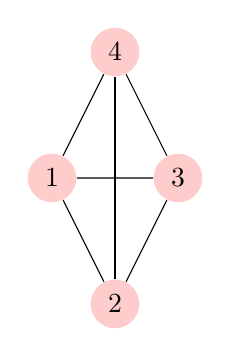
\begin{tikzpicture}
  [scale=.4,auto=left,every node/.style={circle,fill=red!20}]
  \node (n1) at (1,7) {1};
  \node (n2) at (3,3)  {2};
  \node (n3) at (5,7)  {3};
  \node (n4) at (3,11)  {4};

  \foreach \from/\to in {n1/n2,n2/n3,n2/n4,n1/n4,n3/n4,n1/n3}
    \draw (\from) -- (\to);

\end{tikzpicture}
\caption{ Drawing of $K_4$ in which edges cross}\label{9g1}
\end{center}
\end{figure}
\begin{figure}
\begin{center}
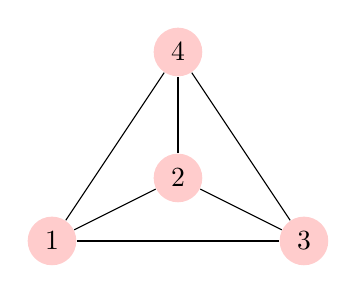
\begin{tikzpicture}
  [scale=.4,auto=left,every node/.style={circle,fill=red!20}]
  \node (n1) at (-1,7) {1};
  \node (n2) at (3,9)  {2};
  \node (n3) at (7,7)  {3};
  \node (n4) at (3,13)  {4};

  \foreach \from/\to in {n1/n2,n2/n3,n2/n4,n1/n4,n3/n4,n1/n3}
    \draw (\from) -- (\to);

\end{tikzpicture}
\caption{ Planar Drawing of $K_4$}\label{9g2}
\end{center}
\end{figure}
 Rishnak showed another graph \ref{9g3} asked Ajur whether he can draw with no edges crossing.
 \begin{figure}
\begin{center}
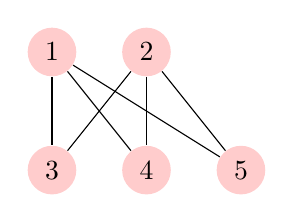
\begin{tikzpicture}
  [scale=.3,auto=left,every node/.style={circle,fill=red!20}]
  \node (n1) at (1,7) {1};
  \node (n2) at (5,7)  {2};
  \node (n3) at (1,2)  {3};
  \node (n4) at (5,2) {4};
  \node (n5) at (9,2)  {5};
 
  
   \foreach \from/\to in {n1/n3,n1/n4,n1/n5,n2/n3,n2/n4,n2/n5}
    \draw (\from) -- (\to);
    \end{tikzpicture}
\caption{ A Bipartite Graph with 5 vertices and 6 edges, denoted by $K_{2,3}$ where the edges cross}\label{9g3}
\end{center}
\end{figure}
Ajur thought for a while and found it a bit challenging. Then he thought of moving the vertex 2 down in which case no edges will cross. He drew the graph as shown in Figure \ref{9g4}
\begin{figure}
\begin{center}
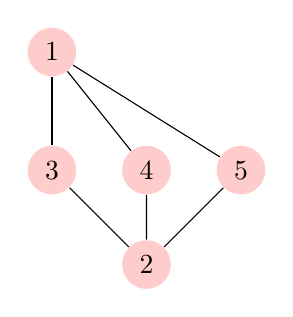
\begin{tikzpicture}
  [scale=.3,auto=left,every node/.style={circle,fill=red!20}]
  \node (n1) at (1,7) {1};
  \node (n2) at (5,-2)  {2};
  \node (n3) at (1,2)  {3};
  \node (n4) at (5,2) {4};
  \node (n5) at (9,2)  {5};
 
  
   \foreach \from/\to in {n1/n3,n1/n4,n1/n5,n2/n3,n2/n4,n2/n5}
    \draw (\from) -- (\to);
    \end{tikzpicture}
\caption{ Planar Drawing of a Bipartite Graph ($K{2,3}$ with 5 vertices and 6 edges with  no edge crossing}\label{9g4}
\end{center}
\end{figure}

Rishnak was impressed. Rishnak asked Ajur if two graphs $G$ and $H$ are isomorphic and if $G$ is planar, can you say $H$ is planar. Ajur said if $H$ is isomorphic to $G$, then each vertex corresponds to some vertex of $G$. By just relabeling the vertices of $G$ in its planar drawing, we get a planar drawing of $H$.
